% Copyright 2006 by Till Tantau
%
% This file may be distributed and/or modified
%
% 1. under the LaTeX Project Public License and/or
% 2. under the GNU Free Documentation License.
%
% See the file doc/generic/pgf/licenses/LICENSE for more details.


\section{Three Dimensional Drawing Library}

\begin{tikzlibrary}{3d}
    This package provides some styles and options for drawing three dimensional
    shapes.
\end{tikzlibrary}
%
\begin{codeexample}[setup code,hidden]
    \usetikzlibrary{3d}
\end{codeexample}


\subsection{Coordinate Systems}

\begin{coordinatesystem}{xyz cylindrical}
    The |xyz cylindrical| coordinate system allows to you specify a point in
    terms of cylindrical coordinates, sometimes also referred to as cylindrical
    polar coordinates or polar cylindrical coordinates. It is very similar to
    the |canvas polar| and |xy polar| coordinate systems with the difference
    that you provide an elevation over the $xy$-plane using the |z| key.
    %
    \begin{key}{/tikz/cs/angle=\meta{degrees} (initially 0)}
        The angle of the coordinate interpreted in the ellipse whose axes are
        the $x$-vector and the $y$-vector.
    \end{key}
    %
    \begin{key}{/tikz/cs/radius=\meta{number} (initially 0)}
        A factor by which the $x$-vector and $y$-vector are multiplied prior to
        forming the ellipse.
    \end{key}
    %
    \begin{key}{/tikz/cs/z=\meta{number} (initially 0)}
        Factor by which the $z$-vector is multiplied.
    \end{key}
    %
\begin{codeexample}[]
\begin{tikzpicture}[->]
  \draw (0,0,0) -- (xyz cylindrical cs:radius=1);
  \draw (0,0,0) -- (xyz cylindrical cs:radius=1,angle=90);
  \draw (0,0,0) -- (xyz cylindrical cs:z=1);
\end{tikzpicture}
\end{codeexample}
    %
\end{coordinatesystem}

\begin{coordinatesystem}{xyz spherical}
    The |xyz spherical| coordinate system allows you to specify a point in
    terms of spherical coordinates.
    %
    \begin{key}{/tikz/cs/radius=\meta{number} (initially 0)}
        Factor by which the $x$-, $y$-, and $z$-vector are multiplied.
    \end{key}
    %
    \begin{key}{/tikz/cs/latitude=\meta{degrees} (initially 0)}
        Angle of the coordinate between the $y$- and $z$-vector, measured from
        the $y$-vector.
    \end{key}
    %
    \begin{key}{/tikz/cs/longitude=\meta{degrees} (initially 0)}
        Angle of the coordinate between the $x$- and $y$-vector, measured from
        the $y$-vector.
    \end{key}
    %
    \begin{key}{/tikz/cs/angle=\meta{degrees} (initially 0)}
        Same as |longitude|.
    \end{key}
    %
\begin{codeexample}[]
\begin{tikzpicture}[->]
  \draw (0,0,0) -- (xyz spherical cs:radius=1);
  \draw (0,0,0) -- (xyz spherical cs:radius=1,latitude=90);
  \draw (0,0,0) -- (xyz spherical cs:radius=1,longitude=90);
\end{tikzpicture}
\end{codeexample}
    %
\end{coordinatesystem}


\subsection{Coordinate Planes}

Sometimes drawing with full three dimensional coordinates is not necessary and
it suffices to draw in two dimensions but in a different coordinate plane.  The
following options help you to switch to a different plane.


\subsubsection{Switching to an arbitrary plane}

\begin{key}{/tikz/plane origin=\meta{point} (initially {(0,0)})}
    Origin of the plane.
\end{key}

\begin{key}{/tikz/plane x=\meta{point} (initially {(1,0)})}
    Unit vector of the $x$-direction in the new plane.
\end{key}

\begin{key}{/tikz/plane y=\meta{point} (initially {(0,1)})}
    Unit vector of the $y$-direction in the new plane.
\end{key}

\begin{key}{/tikz/canvas is plane}
    Perform the transformation into the new canvas plane using the units above.
    Note that you have to set the units \emph{before} calling
    |canvas is plane|.
    %
\begin{codeexample}[]
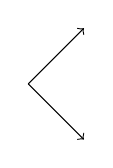
\begin{tikzpicture}[
    ->,
    plane x={(0.707,-0.707)},
    plane y={(0.707,0.707)},
    canvas is plane,
]
    \draw (0,0) -- (1,0);
    \draw (0,0) -- (0,1);
\end{tikzpicture}
\end{codeexample}
    %
\end{key}


\subsubsection{Predefined planes}

\begin{key}{/tikz/canvas is xy plane at z=\meta{dimension}}
    A plane with
    %
    \begin{itemize}
        \item |plane origin={(0,0,|\meta{dimension}|)}|,
        \item |plane x={(1,0,|\meta{dimension}|)}|, and
        \item |plane y={(0,1,|\meta{dimension}|)}|.
    \end{itemize}
\end{key}

\begin{key}{/tikz/canvas is yx plane at z=\meta{dimension}}
    A plane with
    %
    \begin{itemize}
        \item |plane origin={(0,0,|\meta{dimension}|)}|,
        \item |plane x={(0,1,|\meta{dimension}|)}|, and
        \item |plane y={(1,0,|\meta{dimension}|)}|.
    \end{itemize}
\end{key}

\begin{key}{/tikz/canvas is xz plane at y=\meta{dimension}}
    A plane with
    %
    \begin{itemize}
        \item |plane origin={(0,|\meta{dimension}|,0)}|,
        \item |plane x={(1,|\meta{dimension}|,0)}|, and
        \item |plane y={(0,|\meta{dimension}|,1)}|.
    \end{itemize}
\end{key}

\begin{key}{/tikz/canvas is zx plane at y=\meta{dimension}}
    A plane with
    %
    \begin{itemize}
        \item |plane origin={(0,|\meta{dimension}|,0)}|,
        \item |plane x={(0,|\meta{dimension}|,1)}|, and
        \item |plane y={(1,|\meta{dimension}|,0)}|.
    \end{itemize}
\end{key}

\begin{key}{/tikz/canvas is yz plane at x=\meta{dimension}}
    A plane with
    %
    \begin{itemize}
        \item |plane origin={(|\meta{dimension}|,0,0)}|,
        \item |plane x={(|\meta{dimension}|,1,0)}|, and
        \item |plane y={(|\meta{dimension}|,0,1)}|.
    \end{itemize}
\end{key}

\begin{key}{/tikz/canvas is zy plane at x=\meta{dimension}}
    A plane with
    %
    \begin{itemize}
        \item |plane origin={(|\meta{dimension}|,0,0)}|,
        \item |plane x={(|\meta{dimension}|,0,1)}|, and
        \item |plane y={(|\meta{dimension}|,1,0)}|.
    \end{itemize}
\end{key}


\subsection{Examples}

\begin{codeexample}[]
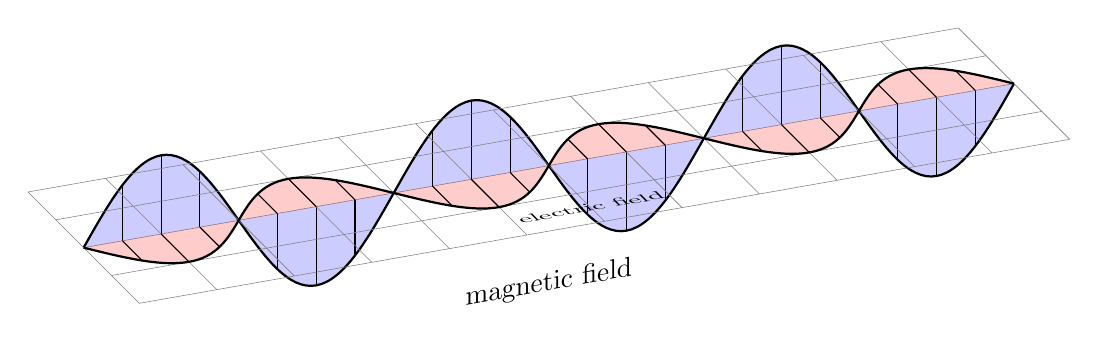
\begin{tikzpicture}[z={(10:10mm)},x={(-45:5mm)}]
  \def\wave{
    \draw[fill,thick,fill opacity=.2]
     (0,0) sin (1,1) cos (2,0) sin (3,-1) cos (4,0)
           sin (5,1) cos (6,0) sin (7,-1) cos (8,0)
           sin (9,1) cos (10,0)sin (11,-1)cos (12,0);
    \foreach \shift in {0,4,8}
    {
      \begin{scope}[xshift=\shift cm,thin]
        \draw (.5,0)  -- (0.5,0 |- 45:1cm);
        \draw (1,0)   -- (1,1);
        \draw (1.5,0) -- (1.5,0 |- 45:1cm);
        \draw (2.5,0) -- (2.5,0 |- -45:1cm);
        \draw (3,0)   -- (3,-1);
        \draw (3.5,0) -- (3.5,0 |- -45:1cm);
      \end{scope}
    }
  }
  \begin{scope}[canvas is zy plane at x=0,fill=blue]
    \wave
    \node at (6,-1.5) [transform shape] {magnetic field};
  \end{scope}
  \begin{scope}[canvas is zx plane at y=0,fill=red]
    \draw[help lines] (0,-2) grid (12,2);
    \wave
    \node at (6,1.5) [rotate=180,xscale=-1,transform shape] {electric field};
  \end{scope}
\end{tikzpicture}
\end{codeexample}

\begin{codeexample}[]
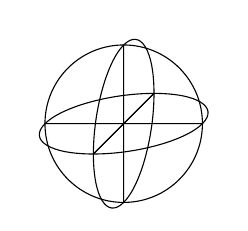
\begin{tikzpicture}
  \begin{scope}[canvas is zy plane at x=0]
    \draw (0,0) circle (1cm);
    \draw (-1,0) -- (1,0) (0,-1) -- (0,1);
  \end{scope}

  \begin{scope}[canvas is zx plane at y=0]
    \draw (0,0) circle (1cm);
    \draw (-1,0) -- (1,0) (0,-1) -- (0,1);
  \end{scope}

  \begin{scope}[canvas is xy plane at z=0]
    \draw (0,0) circle (1cm);
    \draw (-1,0) -- (1,0) (0,-1) -- (0,1);
  \end{scope}
\end{tikzpicture}
\end{codeexample}


%%% Local Variables:
%%% mode: latex
%%% TeX-master: "pgfmanual-pdftex-version"
%%% End:
